%%%%%%%%%%%%%%%%%%%%%%%%%%%%%%%%%%%%%%%%%
% cbio-gres presentation using Execushares
% LaTeX Template
% Version 2.0 (2017-11-20)
%
% Authors: Jackson Antonio do Prado Lima 
% 		  <jacksonpradolima at gmail dot com>
%          Augusto Lopez Dantas
% 		  <aldantas at protonmail dot com>
%
%%%%%%%%%%%%%%%%%%%%%%%%%%%%%%%%%%%%%%%%%

%!TEX program = xelatex
\documentclass[aspectratio=169]{beamer}

%\usepackage[brazil]{babel} % Set the environment to pt-br

%Theme options (allow multiple options):

% Research Group (researchgroup) options: gres (default), cbio, or both
% How to use: \usetheme[researchgroup=cbio]{CbioGres}

% Color theme (colortheme): dark (default), blue, green
% How to use: \usetheme[colortheme=blue]{CbioGres}

\usetheme[colortheme=green,researchgroup=cbio]{CbioGres}

\usepackage{blindtext}
\usepackage{moresize}

\usepackage[ruled,onelanguage]{algorithm2e}
\usepackage[backend=bibtex,style=numeric]{biblatex}
\hypersetup{pdfpagemode=FullScreen}
\bibliography{refs}

\title{Genetic Programming Approach to Deep Neuroevolution}

\author{Ricardo H. R. de Lima \\ Aurora Pozo}

\date{\today}

\subtitle{\tiny{Conference, Month startDay--endDay, Year, City, Country}}

\setcounter{showSlideNumbers}{1}

\begin{document}
	\frame{\titlepage}

	%Agenda
	\begin{frame}		
		\frametitle{Contents}
		\begin{enumerate}
			
			\item Deep Learning \\
				\textcolor{ExecusharesGrey}{\small\hspace{1em} Exploring the topic}
			\item Genetic Programming \\
				\textcolor{ExecusharesGrey}{\small\hspace{1em} Why using it?}
			\item Deep Neuroevolution \\
				\textcolor{ExecusharesGrey}{\small\hspace{1em} Pros and Cons}
			\item Experiments \\
				\textcolor{ExecusharesGrey}{\small\hspace{1em} Initial experiments}
			\item Conclusions \\
				\textcolor{ExecusharesGrey}{\small\hspace{1em} Next steps}
			
		\end{enumerate}
	\end{frame}

	\startprogressbar

%---------------------------------------------------------------------------------------------------
	\section{Deep Learning}
%---------------------------------------------------------------------------------------------------
		\begin{frame}
			\frametitle{Introduction}
			
			\begin{figure}
				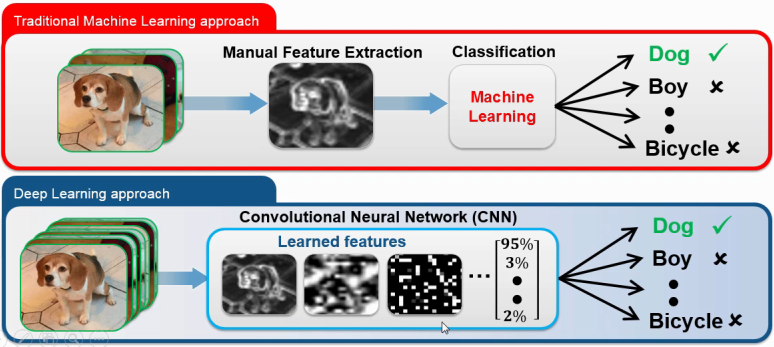
\includegraphics[scale=0.5]{images/dl_example.png}
			\end{figure}

		\end{frame}
%---------------------------------------------------------------------------------------------------
		\begin{frame}
			\frametitle{Introduction}
			
			\begin{block}{}
				Deep Learning is a machine learning technique that can learn \textbf{useful representations} or features directly from images, text and sound
			\end{block}
			
			\begin{itemize}
				\item Machine Learning approach
				\item Learns useful representations or features
				\item Reduces the use of preprocessing
			\end{itemize}

		\end{frame}
%---------------------------------------------------------------------------------------------------
		\begin{frame}
			\frametitle{Convolutional Neural Networks}
			
			\begin{figure}
				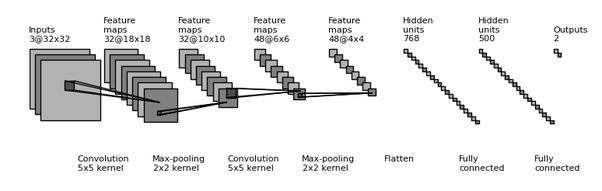
\includegraphics[width=\linewidth]{images/cnn_example.png}
			\end{figure}
		\end{frame}
%---------------------------------------------------------------------------------------------------
		\begin{frame}
			\frametitle{Convolutional Neural Networks}
			
			\begin{figure}
				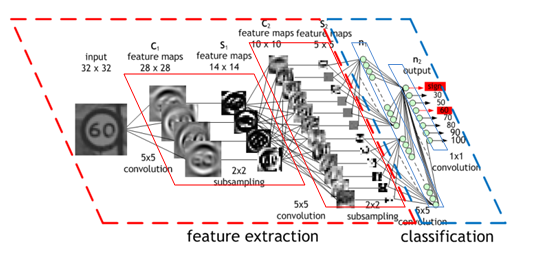
\includegraphics[width=\linewidth]{images/cnn_example2.png}
			\end{figure}
		\end{frame}
%---------------------------------------------------------------------------------------------------
		\begin{frame}
			\frametitle{Convolutional Neural Networks}

			\begin{itemize}
				\item Used for image recognition
				\item Performs both generative and descriptive tasks
			\end{itemize}

			\begin{itemize}
				\item Require large number of examples
				\item High number of trainable parameters
				\item High computational cost
			\end{itemize}

		\end{frame}
%---------------------------------------------------------------------------------------------------
	\section{Genetic Programming}
%---------------------------------------------------------------------------------------------------
		\begin{frame}
			\frametitle{Features}

			\begin{itemize}
				\item Evolve programs
				\item Combines and modifies solutions to create new ones
			\end{itemize}

			\begin{itemize}
				\item Classic Tree-based GP
				\item Grammatical Evolution
				\item Cartesian GP
			\end{itemize}

		\end{frame}
%---------------------------------------------------------------------------------------------------
		\begin{frame}
			\frametitle{Grammatical Evolution}

			\begin{itemize}
				\item BNF Grammar\\
					\textcolor{ExecusharesGrey}{\small\hspace{1em}Define the programs structure}
				\item Mapping process\\
					\textcolor{ExecusharesGrey}{\small\hspace{1em}Translate genotype to phenotype}
				\item Search Engine\\
					\textcolor{ExecusharesGrey}{\small\hspace{1em}Genetic Algorithm}
			\end{itemize}

		\end{frame}
%---------------------------------------------------------------------------------------------------
		\begin{frame}
			\frametitle{Grammatical Evolution}

			\begin{figure}
				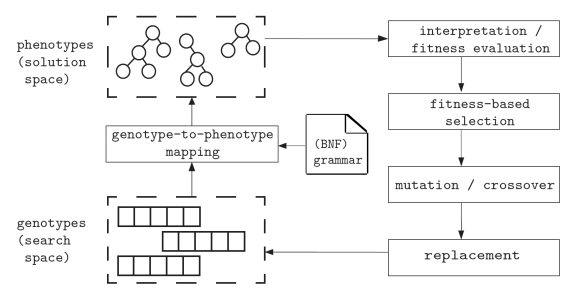
\includegraphics[width=\linewidth]{images/ge_example.png}
			\end{figure}

		\end{frame}
%---------------------------------------------------------------------------------------------------
	\section{Deep Neuroevolution}
%---------------------------------------------------------------------------------------------------
		\begin{frame}
			\frametitle{Proposed Approach}
			
			\begin{block}{}
				Neuroevolution is a form of artificial intelligence that uses \textbf{evolutionary algorithms} to \textbf{generate artifial neural networks}, parameters, topology and rules. Studies on how to evolve Deep Neural Networks are called \textbf{Deep Neuroevolution}
			\end{block}
			
			\begin{itemize}
				\item Fitness function\\
				\textcolor{ExecusharesGrey}{\small\hspace{1em}Accuracy/Error Rate}
				\item Architecture\\
				\textcolor{ExecusharesGrey}{\small\hspace{1em}Define smallest/biggest valid model}
			\end{itemize}
		\end{frame}
%---------------------------------------------------------------------------------------------------
		\begin{frame}
			\frametitle{Approach: Evaluating the Models}
			
			\begin{block}{}
				The CNNs are evaluated using the \textbf{error rate}, obtained from training and test, on well known datasets.
			\end{block}
			
			\begin{itemize}
				\item Number of epochs
				\item Time spent
				\item Loss
			\end{itemize}
			
		\end{frame}
%---------------------------------------------------------------------------------------------------
		\begin{frame}
			\frametitle{Approach: Architecture}
			
			\begin{block}{Smallest CNN}
				The smallest cnn that we can think of is:\\
				inputs >> convolution >> dense >> outputs
			\end{block}
			
			\begin{itemize}
				\item What defines a CNN is the use of convolutions
				\item The NN needs a fully connected layer to process correctly the inputs
			\end{itemize}
			
			\begin{block}{Biggest CNN}
				How many layers is enough? 30, 50, 100?
			\end{block}
			
			\begin{itemize}
				\item Define a upper bound
			\end{itemize}
			
		\end{frame}
%---------------------------------------------------------------------------------------------------
		\begin{frame}
			\frametitle{Approach: Grammar}
			
			\begin{figure}
				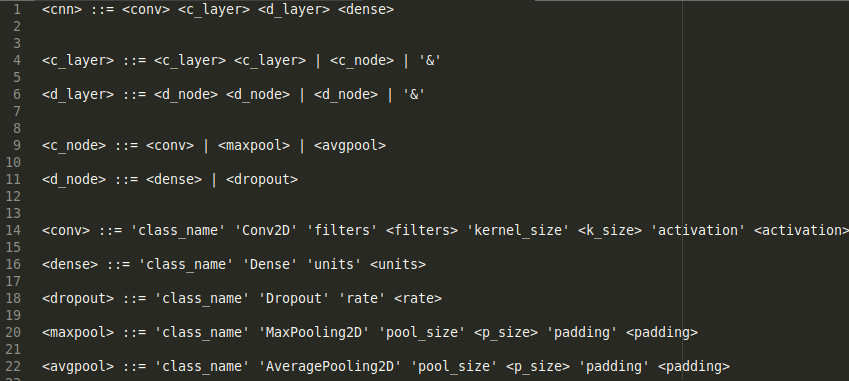
\includegraphics[width=\linewidth]{images/cnn-bnf.png}
				\caption{Part of the proposed grammar for designing CNNs}
			\end{figure}
		\end{frame}
%---------------------------------------------------------------------------------------------------
		\begin{frame}
			\frametitle{Approach: Grammar}
			
			\begin{figure}
				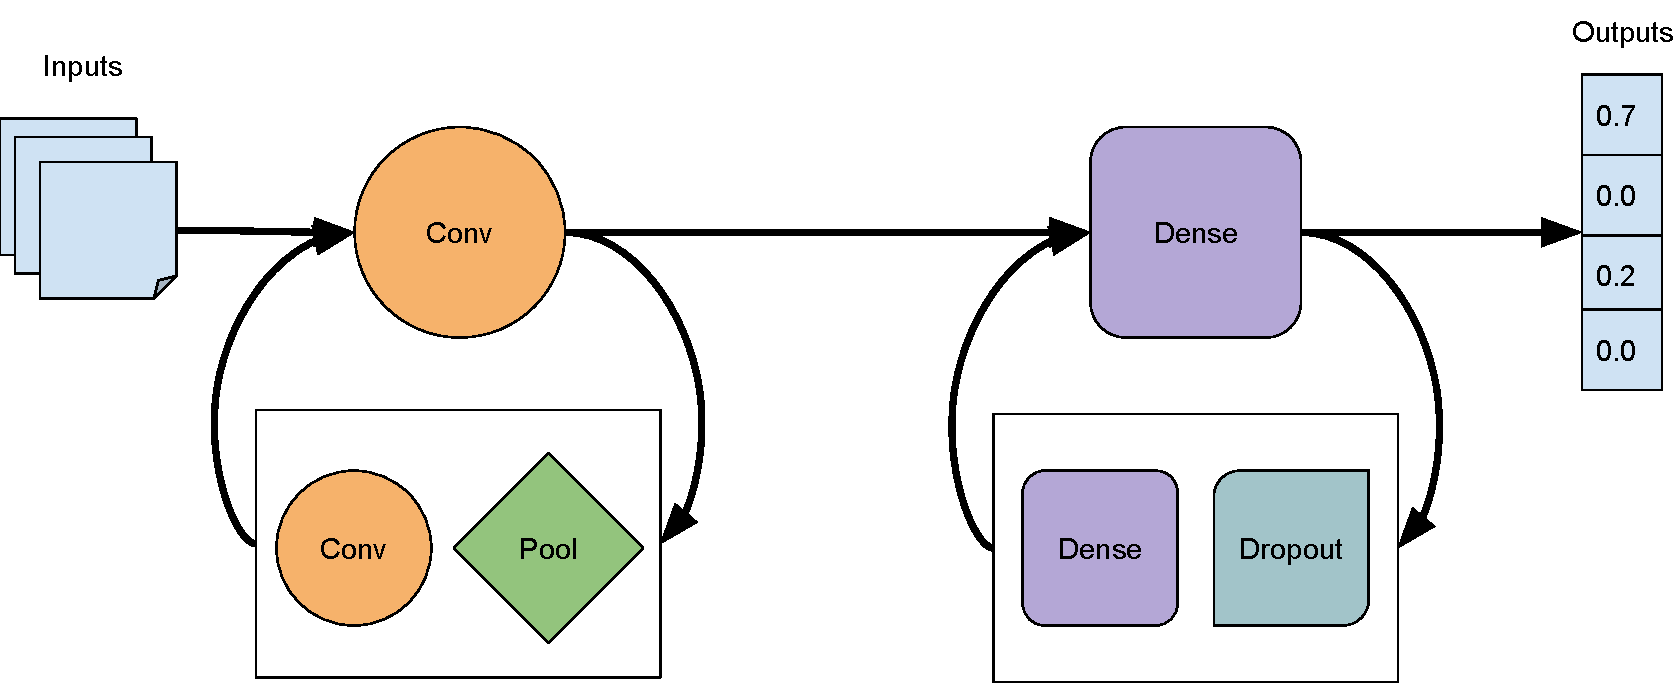
\includegraphics[width=\linewidth]{images/mapping-example.pdf}
			\end{figure}
		\end{frame}
%---------------------------------------------------------------------------------------------------
		\begin{frame}
			\frametitle{Approach: Grammar}
			
			To avoid invalid models, some rules were created:
			
			\begin{enumerate}
				\item All models start with a convolution node
				\item All models end with a dense node
				
				\item The last node has the number of units set to the number of classes
				\item The last node has the activation function set to 'softmax'
				
				\item The first dense node is preceded by a 'flatten' node
			\end{enumerate}
		
			Invalid models are still possible, in these cases, we penalize the solution.
		
		\end{frame}
%---------------------------------------------------------------------------------------------------
		\begin{frame}
			\frametitle{Approach: CNN Parameters}
			
			\begin{itemize}
				\item Convolution: Filters, Kernel Size, Activation
				\item Max/Average Pooling: Pool size, Padding
				\item Dense: Units, Activation
				\item Dropout: Drop rate
				\item Filters: 32, 64
				\item Kernel Size: (3, 3), (5, 5)
				\item Activation: Relu, Tahnm, Linear
				\item Pool size: (2, 2), (4, 4)
				\item Padding: Valid, Same
				\item Units: 32, 64
				\item Drop rate: [0, 1]
			\end{itemize}
		
		\end{frame}
%---------------------------------------------------------------------------------------------------
		\begin{frame}
			\frametitle{Approach: GE Parameters}
			
			\begin{table}
				\begin{tabular}{l|c|c}
					\textbf{Parameter} & \textbf{Method} & \textbf{Value} \\ \hline
					Population         &        -        &       20       \\ \hline
					Evaluations        &        -        &      400       \\ \hline
					Selection          &     Random      &       2        \\ \hline
					Crossover          &    One point    &      0.8       \\ \hline
					Mutation           &      Point      &      0.1       \\ \hline
					Prune              &        -        &      0.1       \\ \hline
					Duplication        &        -        &      0.1       \\ \hline
				\end{tabular}
			\end{table}
		
		\end{frame}
%---------------------------------------------------------------------------------------------------
		\begin{frame}
			\frametitle{Tools}
			\begin{itemize}
				\item Tensorflow/Theano\\
					\textcolor{ExecusharesGrey}{\small\hspace{1em}Powerful tools to build and run cnns}
				\item Keras\\
					\textcolor{ExecusharesGrey}{\small\hspace{1em}High level framework that make easier to build the networks that run over tensorflow/theano}
				\item Python
			\end{itemize}
		\end{frame}
%---------------------------------------------------------------------------------------------------
	\section{Experiments}
%---------------------------------------------------------------------------------------------------
		\begin{frame}
			\frametitle{Experiments: MNIST}

			The MNIST dataset has 50000 for training and 10000 for validation and test. The images are 28x28 greyscale, 10 classes.
			
			\begin{table}
				\begin{tabular}{c|c|c|c|c|c|c|c}
					\hline
					   -    & Run 1 & Run 2 & Run 3 & Run 4 & Run 5 & Mean & Test\\ \hline
					Fitness &   0   &   0   &   0   &   0   &   0   &  0   & 0\\ \hline
				\end{tabular}
			\end{table}

		\end{frame}
%---------------------------------------------------------------------------------------------------
		\begin{frame}
			\frametitle{Experiments: notMNIST}
			
			The MNIST dataset has 50000 for training and 10000 for validation and test. The images are 28x28 greyscale, 10 classes.
			
			\begin{table}
				\begin{tabular}{c|c|c|c}
					\hline
					Run & Solution & Num Params & Test \\ \hline
					Mean & - & 0 & 0 \\ \hline
				\end{tabular}
			\end{table}
		
		\end{frame}
%---------------------------------------------------------------------------------------------------
		\begin{frame}
			\frametitle{Experiments: fashion MNIST}
			
			The MNIST dataset has 50000 for training and 10000 for validation and test. The images are 28x28 greyscale, 10 classes.
		
		\end{frame}
%---------------------------------------------------------------------------------------------------
		\begin{frame}
			\frametitle{Experiments: CIFAR 10}
			
			The MNIST dataset has 40000 for training and 10000 for validation and test. The images are 32x32 RGB, 10 classes.
		
		\end{frame}
%---------------------------------------------------------------------------------------------------
		\begin{frame}
			\frametitle{Experiments: CIFAR 100}
			
			The MNIST dataset has 50000 for training and 10000 for validation and test. The images are 32x32 RGB, 100 classes.
		
		\end{frame}
%---------------------------------------------------------------------------------------------------
	\section{Conclusions}
%---------------------------------------------------------------------------------------------------
		\begin{frame}
			\frametitle{Next steps}
			
			\begin{itemize}
				\item Optimize the Grammar

				\item Add other GP algorithms\\
					\textcolor{ExecusharesGrey}{\small\hspace{1em}Similar work done using Cartesian GP}

				\item Experiments\\
					\textcolor{ExecusharesGrey}{\small\hspace{1em}Verify efficiency of approach}

				\item Compare with similar approaches\\
					\textcolor{ExecusharesGrey}{\small\hspace{1em}CIFAR 10-100/MNIST and other well known datasets}

			\end{itemize}
		\end{frame}
%---------------------------------------------------------------------------------------------------
		\frame{\acknowledgmentpage}
\end{document}